\chapter{V.E.C.T.O.R. -3000}

\begin{figure}[H]
    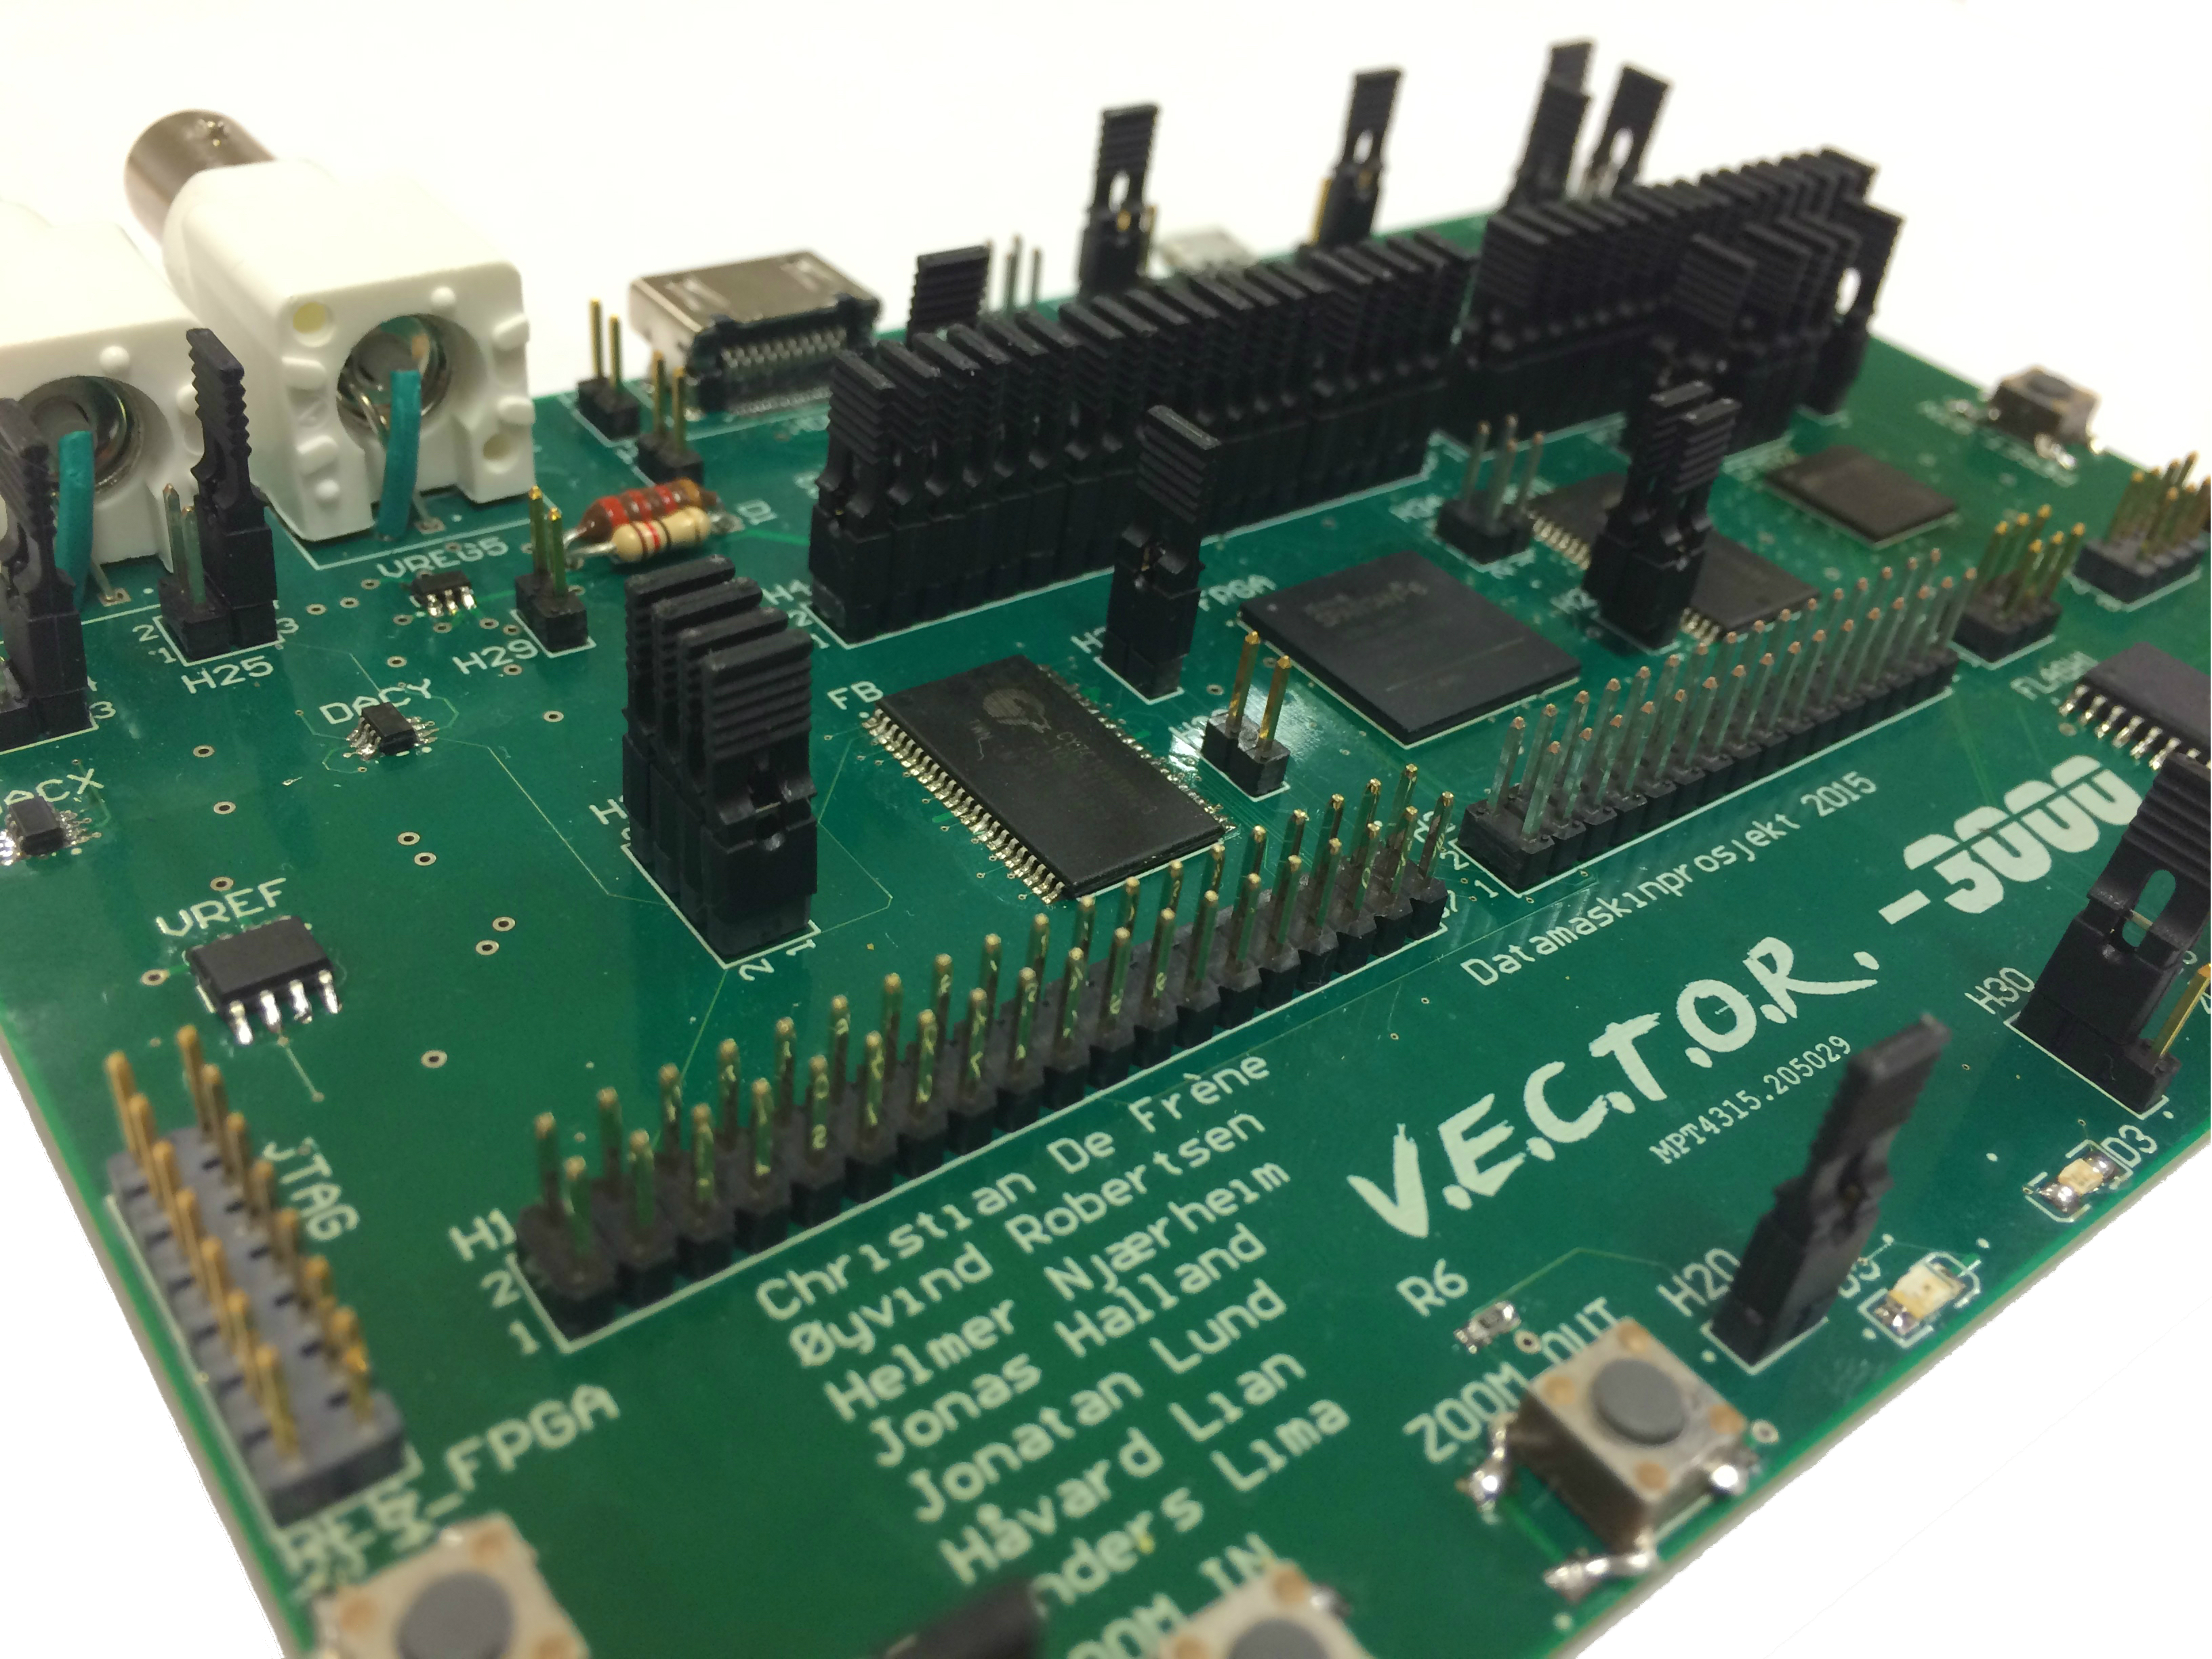
\includegraphics[width=\linewidth]{images/board_angle.jpg}
    \caption{V.E.C.T.O.R. -3000}
    \label{fig:board-angle}
\end{figure}

The end result of the group's work on this project, is a computer architecture made with the processing and production of vector graphics in mind.
Said architecture is named V.E.C.T.O.R -3000, an acronym for Very Efficient Computer for Transferring graphics to Oscilloscope and Raster screens, with the -3000 added as an homage to the retrofuturistic associations of vector graphics in popular culture.

V.E.C.T.O.R. -3000 is a general purpose vector graphics processor, capable of // INSERT MERITS AND FUNCTIONALITY HERE

//TODO: Hvor mye skal vi skrive her egentlig?
